\documentclass[stu,12pt,floatsintext]{apa7}

\usepackage{csquotes}

\usepackage[spanish]{babel}
\usepackage[utf8]{inputenc}

\usepackage[style=apa,sortcites=true,sorting=nyt,backend=biber]{biblatex}
\DeclareLanguageMapping{american}{american-apa}
\addbibresource{bibliografia.bib}

\usepackage[T1]{fontenc} 
\usepackage{mathptmx}
\usepackage{graphicx} 

\title{
  Prevención de errores de hardware y software en dispositivos eléctricos y
  electrónicos por medio de un programa gestor portable
}
\shorttitle{Estado del arte}
\author{Felipe Medina González y Juan David Hernández Palomino}
\duedate{\today}
\affiliation{Universidad Central}
\course{Grupo 1P - Práctica de ingeniería II}
\professor{Dora Janeth Alfondo Cómbita}

\begin{document}
\maketitle
\tableofcontents

\pagebreak
\section{Introducción}

En esta nueva era digital en la que estamos viviendo, la tecnología ha tomado un
rumbo en donde los dispositivos electrónicos y eléctricos se han vuelto
indispensables en la vida diaria ya sea para responder a un jefe, acordar un
evento con unos amigos, entretenerse etc. Y todo esto se considera como una
generación que comenzó desde computadoras de escritorio hasta teléfonos
inteligentes que al menos nacionalmente son mayores que la población total:
``Por citar un simple dato, en el año 2021 en Colombia la población era cercana
a los 47 millones de habitantes y existían aproximadamente 60 millones de
aparatos celulares activos.'' (MinTIC, 2021  como se cita en \cite{Trejos2023})

Estos aparatos otorgan la posibilidad de cumplir con nuestras tareas en los
contextos actuales y ofrecen una cantidad masiva de información. Sin embargo,
detrás de dichas comodidades, se esconden desafíos importantes que lideran y
amenazan el mantener un uso correcto del funcionamiento de estos dispositivos y
la seguridad de nuestros datos. Tales desafíos se caracterizan con encontrar
fallas en los dispositivos que comúnmente se tienen en nuestras casas y que por
norma general al ser bastante complejos, se tiene poco conocimiento de lo que
ocurre tanto a nivel físico (hardware) como a nivel lógico (software) y solo
disponemos de lo que se ve en las pantallas. 

Mantener un computador completamente funcional resulta bastante problemático al
componerse de circuitos eléctricos que con el paso del tiempo pueden
deteriorarse y en el proceso se generan alteraciones muy molestas, como
``artefactos'' en el monitor, que la máquina se apague durante la realización de
una actividad, que de repente el sonido no funcione, que por ninguno de los
medios se puede tener conexión a internet etc.

Estas alteraciones no solo causan inconvenientes y frustración para los
usuarios, sino también alimentan problemas como la obsolescencia tecnológica y
las fallas de hardware. En donde se examina que los dispositivos son desechados
debido a que sus componentes dejan de ser compatibles, no tienen el rendimiento
que se tenía desde su fabricación o simplemente dejan de funcionar por un
problema físico del que los usuarios tienen control nulo. Estas situaciones
obligan a los usuarios a tener que hacer cambios en la máquina que se tiene,
pero aquello representa un gasto significativo para una organización que cuente
con varios dispositivos, y ni hablar de los usuarios domésticos.

Este ciclo constante de reemplazo surge de la necesidad de una solución integral
que aborde tanto el mantenimiento preventivo de hardware y software de la mano
con la ciberseguridad. Siendo esta última una cuestión que resulta preocupante,
pues no solo deja comprometido el estado de los archivos de un equipo, sino que
también puede influir en otros aspectos como la economía, movimientos sociales,
aspectos ecológicos o la integridad total de una maquinaria pensada para operar
con elementos masivos, como las fábricas.

Ante estas dos cuestiones y sumado a la necesidad del mundo actual de tener
conocimiento de las cosas que hay alrededor, surgió la idea de crear una
aplicación que pueda otorgar conocimiento de los elementos que son problemáticos
tanto en el hardware, como de la seguridad de la información de un dispositivo
de cómputo, siendo esta última una cuestión que cada vez evoluciona de acuerdo a
los problemas que surgen ante el control de la información que se desea
almacenar.

\pagebreak
\section{Problemática}

Una de las cosas que señala \textcite{Jin2023} es que en los circuitos de un
computador se pueden encontrar fallas que se caracterizan principalmente por la
degradación de uso y el estropeo repentino de algún componente. En principio
se piensa que ya se debería tener control de ese aspecto, pero se sigue tratando
de manejar tal situación por la cantidad de demanda por la reparación de
computadores tanto domésticos como empresariales. Además, una de las cosas que
\textcite{Aboaoja2022} aborda sobre la ciberseguridad, que es una de las áreas
más importantes para la protección de la información de los usuarios y que
procura evitar que los sistemas de cómputo tengan fallos

Ambas áreas son enfocadas principalmente debido a su relación que tienen con el
funcionamiento de un equipo de cómputo, ya que si el mismo tiene una deficiencia
en su funcionamiento, bien pueda ser que en la parte física haya un
comportamiento que no deba ocurrir, o que en el software (la parte lógica) tenga 
integrado un elemento que estorbe las acciones que el usuario quiera realizar.
Las situaciones a continuación describen lo que se refiere cuando se habla de
``Inadecuado funcionamiento de un equipo de cómputo'' tanto para dispositivos de
sobremesa como móviles:

\subsection{Situaciones relacionadas con el mal funcionamiento de hardware}

\textcite{Herat2020} informó que en 2019 se observó que alrededor del mundo se
desperdiciaron 53.6 millones de toneladas métricas y que se estimó que para el
2023 se tendrán 74.7 millones de toneladas métricas de desperdicios
electrónicos. Y que anualmente se desechan entre 1 y 10 millones de toneladas
métricas en los países industrializados y los que están en vías de desarrollo
desechan alrededor de 500 mil y un millón de toneladas métricas. Esta
acumulación de dispositivos se generan normalmente por una serie de actitudes
que \textcite{Hartl2023} relacionan con la psicología del mercado cuando las
empresas que fabrican diversos productos que con el paso del tiempo resultan
tener más capacidad, más velocidad y más eficiencia: ``Los bienes duraderos
que se estropean al cabo de un tiempo inducen a los consumidores a comprar uno
nuevo, lo que estimula la demanda de este producto.''

Ante esta situación, Kaliyavaradhan et al. (2022) como se cita en
\textcite{Seif2024} encontraron que esta actitud ocurre principalmente por los
acelerados cambios y avances que presenta la tecnología ante varias de nuestras
actividades cotidianas y laborales, cosa que lleva a directamente hacer
reemplazos constantes debido a las incompatibilidades que presentan las
herramientas de software con los componentes y capacidades del hardware: ``A
medida que entran en el mercado nuevos dispositivos con las últimas
prestaciones, los consumidores se deshacen de los más antiguos, lo que aumenta
las tasas de residuos''

Un aparato electrónico que se estropea de forma inesperada, normalmente uno
podría pensar que el problema viene a través del uso, sin embargo, también se
encontró de acuerdo con \textcite{Hartl2023} que también ocurre por
conveniencia empresarial, ya que si alguien nota que su máquina no funciona
como se espera o deja de ser útil, entonces se cambia para mantener a flote la
economía de la empresa que diseña el producto:

\begin{displayquote}
  Aunque ingenuamente se podría pensar que la vida útil de un producto depende
  normalmente del desgaste de sus materiales más alguna influencia aleatoria,
  también puede ser el resultado de una elección empresarial. La obsolescencia
  planificada significa que las empresas diseñan sus productos de forma que no
  duren mucho.
\end{displayquote}

% Otras cuestiones a tratar
Ahora, en cuanto a los aspectos técnicos sobre las fallas en aspectos de
hardware, en la fabricación se tiene un análisis sobre el funcionamiento del
circuito usando un modelo lógico de fallos y otro de simulación de sistemas. Pero
como somos seres que cometen errores, a la hora de hacer tales análisis se
omiten ciertos datos particulares como la implicación que podrían generar
ciertos componentes tras haber realizado en un componente en particular o el
resultado que se generó tras el diseño de las partes que conforman los equipos
de cómputo. \parencite{Jin2023}

En esto da sentido a lo que expresan \textcite{Zailani2021} cuando se
encuentran con la problemática de que los usuarios que no son experimentados en
la mantención de hardware y deciden tomar las medidas que solo conocen, pero
que resultan ineficientes ante las situaciones que se presentan cuando un
dispositivo tiende a fallar por algún motivo: 

\begin{displayquote}
  A veces, algunos productos informáticos del mercado ofrecen lugares de
  servicio oficiales de difícil acceso, por lo que los usuarios se muestran
  reticentes a repararlos y, al final, prefieren los lugares de servicio
  públicos. Sin embargo, algunos usuarios saben que si reparan su ordenador en
  un lugar público, es arriesgado porque no hay información clara sobre los
  costes de reparación ni sobre los daños.
\end{displayquote}

\subsection{Situaciones relacionadas con las fallas de ciberseguridad}

Por norma general, algunas veces vemos que ``ciberseguridad'' y ``seguridad
informática'' son sinónimos. Sin embargo, la seguridad informática es el área de
proteger la información de los riesgos que conlleva el entorno en donde se
encuentra y que puede tener otros formatos que no siempre están relacionados
con los equipos de cómputo. En cuanto a la ``ciberseguridad'' tiene una cuestión
similar, solo que se especializa en la protección datos almacenados en sistemas
de cómputo; lo que significa que la ciberseguridad hace parte de la seguridad
informática: ``Se entiende que la ciberseguridad tiene como objetivo
principal la protección de la información digital, que está o es transmitida
entre los todos los dispositivos que se encuentran interconectados, por esto,
la ciberseguridad está en la seguridad informática''
\parencite{Mosquera2019} 

Así que reconociendo lo que representa la ``ciberseguridad'' y teniendo en
cuenta que esto se aplica a diversas áreas como lo comenta
\textcite{CanoMartinez2022} de que la seguridad de la información digital es
primordial, ya que si es escasa, se pueden generar desde efectos molestos hasta
destructivos en el aspecto político, económico, legal, etcétera:

\begin{displayquote}
  En este escenario, la ciberseguridad nacional enfrenta diferentes tensiones y
  fuerzas a nivel político, económico, social, tecnológico, legal y ecológico,
  que demandan salir de la postura tradicional de “esperar y ver”, para
  movilizar reflexiones y esfuerzos que permitan “delinear y actuar”.
\end{displayquote}

Sabiendo que en diversos entornos, se pueden encontrar brechas que pueden ser
aprovechables tanto por cualquier persona como de cualquier otro software. Una
de las partes más preocupantes es el hecho de que los ransomware (malware que
cifra datos) sea el tipo de malware que actualmente es uno de los que son más
frecuentes: ``El Netskope Cloud Report de septiembre de 2016 reveló que el
55,9\% de los archivos infectados con malware que se encuentran en las
aplicaciones en la nube se comparten públicamente, por lo que la nube es una
plataforma atractiva para los atacantes.'' \parencite{Rosli2019}

Los mismos demuestran que los problemas en cuanto a malware cada
vez se hacen más notorios, por ejemplo en la Figura~\ref{fig:report2017} se
muestra de forma general la cantidad de incidentes relacionados con la
ciberseguridad en 2018. Y los mismos también comentan que la tasa del malware
aumentó a un 43.5\% del total de los incidentes ocurridos en 2018. Lo que indica
qué tan importante es el de hacer que los usuarios se encuentren con malware.

\begin{figure}[htb]
  \centering
  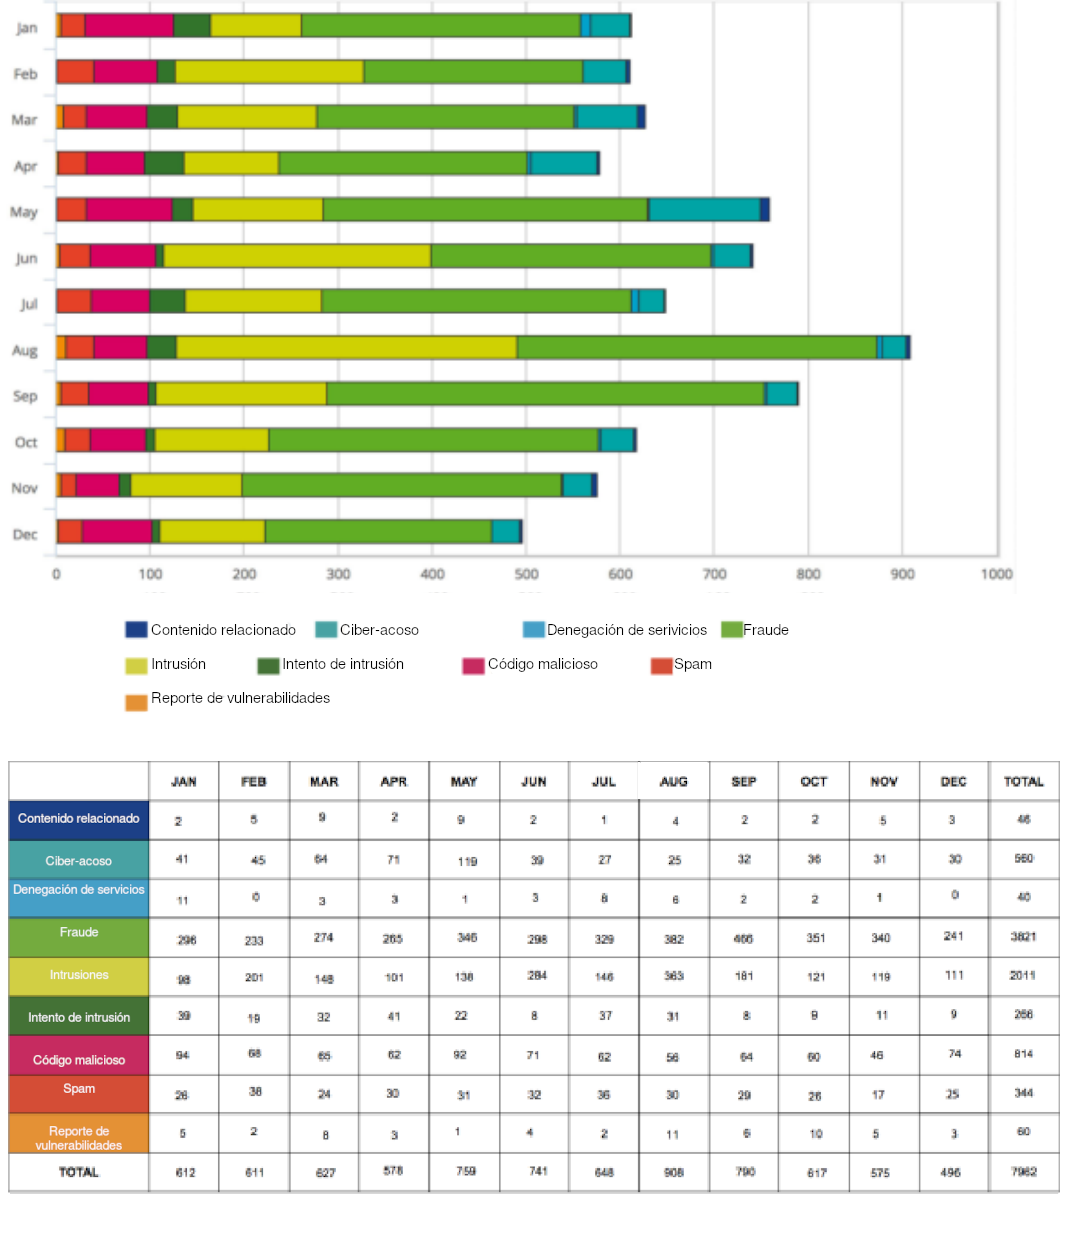
\includegraphics[width=0.75\textwidth]{./pictures/report2017.png}
  \caption{
    \textbf{Nota:} Estadísticas de incidentes reportados en 2017 Tomado de
    \cite{Rosli2019}
  }
  \label{fig:report2017}
\end{figure} 

% Otro problema para otros entornos

\subsubsection{Problemas en el aspecto de los sistemas de salud}

Una de las áreas en las que también se logra presenciar lo comprometidas que se
encuentra la ciberseguridad en los sistemas sanitarios al quedar completamente
expuestos; una prueba realizada por Google, se descubrió que una de sus
inteligencias encontraron y expusieron información crítica tanto de médicos
como de pacientes. Lo que significa que los ``cibercriminales'' pueden realizar
sus objetivos relacionados con el sistema sanitario:

\begin{displayquote}
  Informes aparecidos en el Washington Post y en otros medios de comunicación
  han descrito cómo las asociaciones de Google con el fin de entrenar algoritmos
  de inteligencia artificial dieron lugar inadvertidamente a que algunos datos
  con información sanitaria protegida se cargaran de forma que quedaran
  expuestos a cualquier persona con una capacidad básica de motor de búsqueda.
  \parencite[Wakabayashi D, 2019, como se cita en][]{Banja2020}
\end{displayquote}

También \textcite{Banja2020} destacó que en diversas organizaciones se almacene
información de manera consentida, por lo que si hay fallas de seguridad por
parte de un ente, (no tiene que ser necesariamente un atacante) se compromete
entonces el estado de seguridad de la gente a la que pertenece tal entidad. Y
también 

% Poner sus mejoras
\subsubsection{Problemas en el IoT}

A grandes rasgos, es un campo en el que objetos de uso cotidiano están
conectados a una red, que a su vez, está conectada a internet. A pesar de ser un
campo en el que es poco común en el uso diario, se vuelve completamente
importante en la seguridad informática, ya que como comenta
\textcite{Aboaoja2022}, el desarrollo del malware se volvió tan sofisticado que
los que terminan siendo desarrollados pueden distinguir el tipo de máquina en
la que están, así que no es de extrañar que existan programas que se dispersen
en una red sin el consentimiento de los usuarios.

En el Internet de las Cosas al estar repleto de tantos computadores, se requiere
entonces de una cantidad de recursos masiva para la protección de la información
que se utiliza, y como el malware cada vez se hace más silencioso ante la
protección, cosa que es my peligroso para entidades que usan el IoT de forma
común y se tenga que gastar más 6.000 millones de dólares para sistemas de
protección de la información bastante avanzados:

\begin{displayquote}
  Los informes de Gartner1 y Juniper Research2 sugieren que el gasto mundial en
  seguridad de IoT fue de 1.1 mil millones de dólares y se disparó más de 3.1
  mil millones de dólares en 2021. Además, se prevé que se dispare hasta los
  6.000 millones de dólares en 2023, lo que es un resultado directo del aumento
  de las vulnerabilidades en los sistemas. La discusión anterior nos lleva a
  creer que el diagnóstico y la resolución de fallas en un sistema IoT será un
  gran problema en el futuro cercano, a menos que todas las entidades dentro del
  sistema pertenezcan a la misma empresa. \parencite{Singh2022}
\end{displayquote}

\subsubsection{Situaciones nacionales}

\textcite{CanoMartinez2022} y \textcite{Mosquera2019} muestran lo que ocurre a
nivel nacional sobre el estado de la seguridad informática y no únicamente
viendo los delitos que más se cometieron con respecto a lo que se muestra en la
Figura~\ref{fig:delitos} de acuerdo con la Ley 1273 de 2009 del código penal
nacional. Aunque aquello pone en evidencia que se procura obtener un beneficio
comercial o económico, ellos también evidencian que se realizan para tener una
influencia sobre las actividades comunes. Siendo estas extendidas al uso de las
tecnologías de forma amplia.

\begin{figure}[htb]
  \centering
  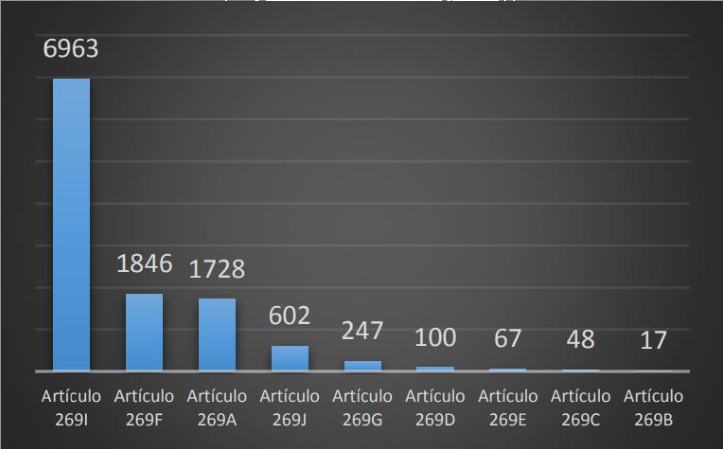
\includegraphics[width=0.75\textwidth]{./pictures/delitos.png}
  \caption{
    \textbf{Nota:} Esta gráfica representa el delito más denunciado según el
    balance del cibercrimen en Colombia en 2017, donde se habían recibido
    11.618 denuncias. Tomado de \cite{Mosquera2019}
  }
  \label{fig:delitos}
\end{figure}

\textcite{He2023}

\subsection{Diagrama de Ishikawa y conclusiones generales de los problemas}

% Por completar
\textcite{CanoMartinez2022} junto con los comentarios dados por
\textcite{Nurul2021} se identificó que la causa más común de las fallas de
seguridad de un sistema tecnológico es el engaño; independientemente de las
técnicas de ``hacking'' que se empleen, se puede llegar a lo que se desea de
una o varias personas.

Al tener en cuenta varias de las causas que provocan el inadecuado
funcionamiento de un equipo de cómputo, se sintetizan en la
Figura~\ref{fig:fish}:

\begin{figure}[htb]
  \centering
  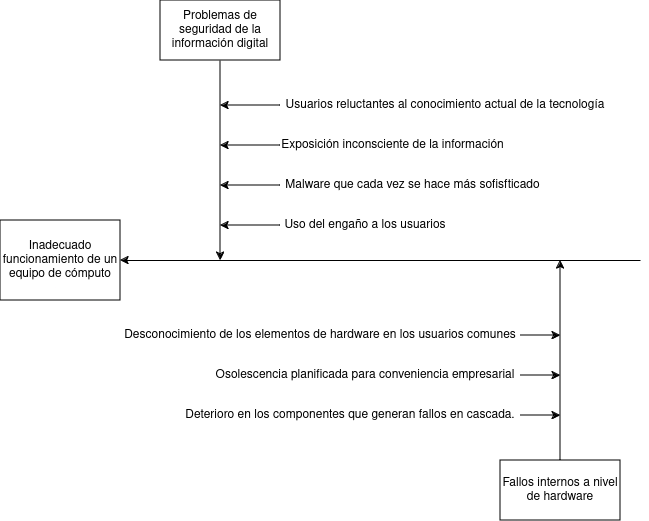
\includegraphics[width=0.9\textwidth]{./pictures/diagrama.png}
  \caption{Diagrama de Ishikawa sobre la problemática}
  \label{fig:fish}
\end{figure} 

\pagebreak
\section{Justificación}

Pese a lo que \textcite{Herat2020} detalla sobre las soluciones proporcionadas
por las empresas, \textcite{Hartl2023} encontraron que no todas las personas son
conscientes de este hecho, y por ende sus productos se añaden a los valores de
los desperdicios eléctricos y electrónicos que \textcite{Seif2024} menciona de
forma general. Considerando que en la mayoría de los casos se asegura un periodo
de tiempo para mantener a flote la economía de las firmas, al ver que los
usuarios tienen el deseo de comprar un aparato electrónico de mayor calidad una
vez se presentan fallos. Sin embargo, no todos se encuentran con la posibilidad
de reemplazar una máquina en periodos de tiempo, en particular si estos son
cortos, cosa que resulta costosa para los usuarios.

Y no solo en los fallos físicos por desgaste o los fallos internos inesperados,
sino que como se vieron con las revisiones hechas por \textcite{Rathore2023} o
\textcite{Waqar2023} (En el caso de los dispositivos móviles) sobre el tema de
la ciberseguridad, a los que \textcite{CanoMartinez2022} considera como
primordiales para los aspectos nacionales más importantes como la economía o la
estabilidad de las empresas. Asumiendo que 53.47\% de los usuarios
mayores son engañados por mensajes que ofrecen algo, se consideró que se tiene
que hacer un software que cumpla las características de prevenir al usuario de
malware, además de monitorear y analizar el rendimiento del equipo para su
mantenimiento preventivo. Todo esto junto con una guía del lenguaje que se tiene
sobre los sistemas informáticos actuales de tal modo que, como lo sugiere
\textcite{Nurul2021}, se pueda tener una idea sobre cómo las aplicaciones y el
software a desarrollar funcionan en los equipos de cómputo. 

Por lo tanto, la idea de la aplicación a desarrollar se basa principalmente en
reducir los riesgos que se generan, y según lo expresa \textcite{Mosquera2019},
al realizar varias de las actividades que involucran directamente el
desconocimiento de la información que se suele presentar por parte los nuevos
usuarios, muchos atacantes aprovechan los vacíos de seguridad que los presenta
y por ende, hacerlos quedar expuestos a varias amenazas que atentan con la
privacidad, la identidad, el estado de una organización o las infraestructuras
críticas. \parencite[e.g.,][]{CanoMartinez2022} 

\pagebreak
\section{Estado del arte}

Al basarse en los autores consultados, pueden identificar varios conceptos y
técnicas que manejan la ciberseguridad y el mantenimiento preventivo de equipos
de una forma experimental, es decir, que se basan en qué tan efectivas son en
sus campos y se obtuvieron una colección de elementos a tratar. La idea de
tales aportes consiste principalmente en reducir los fallos, ya que como
menciona \textcite{Rathore2023} es imposible que un sistema esté sin errores,
pero es posible reducir su cantidad.

Esto se procura hacer, puesto que independientemente de qué tan sofisticados y
modernos que sean los sistemas de información, siempre se van a encontrar fallas
potenciales y son tan impredecibles como lo son el ver que un equipo deje de
funcionar: ``Dada la necesidad de actualizaciones constantes, la posibilidad de
que se produzcan nuevos fallos en el sistema está siempre presente, con
frecuencia es imprevisible y a veces imposible de prevenir.''
\parencite{Banja2020}

Las revisiones experimentales emplearon técnica que definen el estado actual
del mantenimiento preventivo de equipos tanto de hardware como de software en
la perspectiva de la seguridad, como la extracción de características de un
Malware, el aprendizaje por refuerzo de una inteligencia basada en Machine
Learning, la funcionalidad de un malware, etcétera.

\subsection{Estado de la técnica del mantenimiento preventivo}

Reconociendo los aportes dados por Vieras (2011) como
se cita en \cite{Zambrano2020}, se puede sobreentender el mantenimiento
preventivo como lo que realiza un servicio técnico con los usuarios.

\subsubsection{Machine Learning}

Como tal, su objetivo es automatizar la tarea de construcción de modelos
analíticos para realizar tareas cognitivas como la detección de objetos o la
traducción de lenguaje natural. Esto se consigue aplicando algoritmos que
aprenden iterativamente a partir de datos de entrenamiento específicos del
problema, lo que permite a los ordenadores encontrar ideas ocultas y patrones
complejos sin ser programados explícitamente.
\parencite[Bishop, 2006  como se cita en][]{Janiesch2021}

En la Figura~\ref{fig:venn_diagram} se logra comprender la forma en la
que está constituido el Machine Learning, sobre todo, para distinguer el también 
el llamado Deep Learning que de acuerdo con las mismas fuentes, se considera un
tipo de aprendizaje que requiere de una maquinaria mucho más pesada de lo normal,
es decir que requiere de un coste computacional (memoría, energía y
procesamiento) mucho mayor de lo habitual, por eso es muy común ver su
funcionamiento en servidores y generadores de imágenes:

\begin{displayquote}
  En cambio, los modelos demasiado complejos entrañan un mayor riesgo de
  sobreajuste. Además, su razonamiento es más difícil de interpretar y es
  probable que sean más costosos desde el punto de vista informático. Los
  costes computacionales se expresan mediante los requisitos de memoria y el
  tiempo de inferencia para ejecutar un modelo en datos nuevos. Estos criterios
  son especialmente importantes a la hora de evaluar las redes neuronales
  profundas, en las que pueden procesarse y almacenarse varios millones de
  parámetros del modelo, lo que impone exigencias especiales a los recursos de
  hardware. \parencite{Janiesch2021}
\end{displayquote}

\begin{figure}[htb]
  \centering
  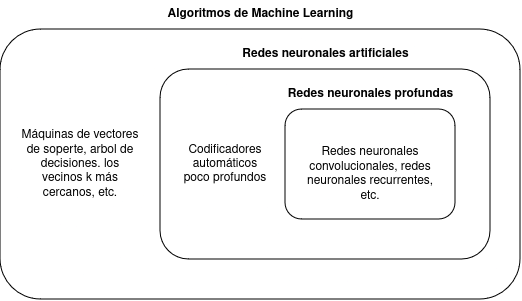
\includegraphics[width=0.75\textwidth]{./pictures/venn_diagram.png}
  \caption{
    \textbf{Nota:} Diagrama de Venn de los conceptos y clases del Machine
    Learning. Tomado de \cite{Janiesch2021}
  }
  \label{fig:venn_diagram}
\end{figure}

Para describir cómo funciona, \textcite{Janiesch2021} comentan que esta
inteligencia se utilizan las tres técnicas fundamentales en donde se aplica su
uso: ``En función del problema planteado y de los datos disponibles, podemos
distinguir tres tipos de Machine Learning: aprendizaje supervisado, aprendizaje
no supervisado y aprendizaje por refuerzo.''

\begin{itemize}
  \item \textbf{Aprendizaje supervisado:}
    Por norma general, \textcite{Janiesch2021} lo definen como una serie de datos
    preexistentes los cuales le sirven a la inteligencia para tener criterio tanto
    de elementos de entrada, como de salida de un sistema que muchas veces es un
    software que se dedica a recopilar información; por ejemplo, de una base de
    datos que almacena suscripciones de un sitio web cualesquiera.

  \item \textbf{No supervisado:}
    Esta técnica en el contexto de intentar encontrar anomalías en un sistema
    individual o un conjunto de estos, se refiere como la detección de patrones
    sin necesidad de información a priori y al aprendizaje se realiza al
    identificar un ``factor común'' de grupos que conforman la información que la
    inteligencia recibe: ``Machine Learning se define como ``la adquisición de una
    descripción estructural a partir de ejemplos''. Esta descripción puede
    utilizarse para inferir reglas de clasificación (u otro tipo de reglas no
    supervisadas, por ejemplo, reglas de agrupación)''.
    \parencite[Witten et al., 2011, como se cita en][]{Singh2022}

  \item \textbf{Aprendizaje por refuerzo:}
    Cuando la inteligencia está con cierto grado de criterio gracias al aprendizaje
    supervisado y con la funcionalidad implementada en el aprendizaje no
    supervisado, se utiliza entonces el aprendizaje por refuerzo para poder ampliar
    nuevos conocimientos y habilidades a través de ``recompensas'' y ``castigos'',
    los cuales hacen que la inteligencia tenga una mejor toma de decisiones:

    \begin{displayquote}
      El aprendizaje por refuerzo funciona secuencialmente en un entorno
      realizando una acción, evaluando su recompensa y ajustando las acciones
      siguientes en consecuencia. En concreto, un paradigma de aprendizaje por
      refuerzo implica un agente que observa el entorno y realiza acciones para
      maximizar la recompensa determinada por el problema en cuestión.
      \parencite[Richard S Sutton y Andrew G Barto., 2018, como se cita en][]
      {Chen2023}
    \end{displayquote}

    Los mismos autores mencionan otros elementos clave relacionados con el
    aprendizaje bajo refuerzo tales como el espacio de acción, entorno, estado,
    observaciones y recompensa y política. El espacio de acción se refiere a las
    opciones que puede tomar el agente por medio inteligencia gracias al
    aprendizaje supervisado. \parencite{Janiesch2021}

    El entorno se considera el espacio en donde se puede mover el agente. El
    estado se refiere a las condiciones en las que se presenta el mismo a modo
    de configuración. La recompensa se refiere al mayor beneficio que se puede
    obtener a nivel tras realizar las acciones que se obtienen en el entorno. Y
    la política significa que, dado un estado, la inteligencia por medio del
    agente ha de realizar una serie acciones específicas de acuerdo con sus
    posibilidades. \parencite{Chen2023}
\end{itemize}

\iffalse
\subsubsection{Manejo de dispositivos de IoT}

% mmejorar esta parte

IoT (Internet de las cosas, en inglés) a pesar de no ser una parte muy común,
cada vez en el ámbito tecnológico se vuelve importante, ya que hace un cambio
radical respecto a cómo nos comunicamos y cómo transmitimos la información. 
\textcite{Singh2022} comenta que 
\fi

\subsubsection{Ada Test}

El fundamento de poder explicar lo que es Ada Test, primero 
define los siguientes conceptos conceptos:


Ada test, \textcite{Chen2023} se muestra como un algoritmo de pruebas sobre la
existencia de troyanos de hardware, dicho algoritmo pasa por las siguientes
fases: Fase I (Perfilado de circuitos), Fase II (Generación de patrones de
prueba adaptativos basados en aprendizaje por refuerzo). Tal algoritmo se
propuso como una mejora a los métodos que se emplean para estudiar el estado de
los circuitos integrados de forma que cuando se estén utilizando, se emplee su
desempeño como corresponde, que sea seguro para procesadores de sistemas de
cómputo y que no implique desarmar el circuito para comprobar su funcionamiento.
La manera en como se conoce esto, es a través de los siguientes conceptos que 
\textcite{Chen2023} explicó:

\begin{itemize}
  \item \textbf{Troyano de hardware:}
    Modificaciones maliciosas en el hardware que pueden encontrarse por defecto
    en la cadena de los circuitos integrados de una máquina. Normalmente tiene
    dos características: Payload y gatillo, la primera consiste el efecto del
    circuito que no funciona como debería y la segunda es la señal que determina
    si la payload se ejecutará o no. La Figura~\ref{fig:circuit} utiliza un
    circuito con puertas lógicas AND y XOR que son usadas para gatillo y
    payload respectivamente.

  \item \textbf{Puertas lógicas:}
    Para conocer lo que ocurre en la Figura~\ref{fig:circuit}, tenemos que
    asumir que desde el lado izquierdo, está circulando corriente eléctrica en
    una o más líneas del esquema, que resultan ser las entradas de las puertas
    lógicas; es irrelevante saber por dónde entra la corriente, pues lo
    importante es saber que las puertas lógicas son componentes electrónicos
    que definen si la corriente continua a través de ellas o no. La forma en la
    cual estas puertas definen las decisiones, se basan directamente en
    operadores lógicos en matemáticas (por ejemplo, las puertas AND se
    comportarán como el operador de conjunción, el OR se comportará como el
    operador de disyunción, etc). La Figura~\ref{fig:logic} expresa el
    funcionamiento de tales puertas.

  \item \textbf{Análisis de canal lateral:}
    Es la revisión de troyanos de hardware para determinar si hay un cambio en
    los parámetros físicos (como energía o retarde del trayecto del circuito)
    y para conocer su presencia se utiliza un esquema de circuito bajo prueba
    para comprobar si el troyano directamente hace una modificación en el
    circuito.

  \item \textbf{Pruebas lógicas:}
    Puede detectar troyanos funcionales, es decir aquellos que eliminan y añaden
    otras operaciones de bajo nivel; cambia la funcionalidad básica de las
    operaciones lógicas. El problema de las pruebas lógicas es que involucra
    dejar ciertos caminos que pueden implicar otros circuitos de troyanos de
    hardware parecidos a los de Figura~\ref{fig:circuit}

  \item \textbf{Perfilado de circuitos}
    Es una fase de Ada Test en donde se computa la transición de probabilidades
    de cada nodo y se computa los parámetros de capacidad de prueba del programa
    de Análisis de Controlabilidad/Observabilidad Sandia. Esta fase busca
    principalmente generar un circuito bajo pruebas con el fin de determinar si
    un circuito puede tener troyanos de hardware de la manera en como se espera.

    Computar la transición de probabilidades en cada nodo (puerta lógica) de la
    lista de redes implica en reconocer los elementos de un troyano de hardware
    del mismo. Para realizar tal computación se utiliza un modelo matemático tal
    que así: $ P_{trans} = p(1-p) $ donde $ p $ es resultado de la probabilidad
    de cada nodo y $ P_{trans} $ es comparado con un umbral $ \theta $ para
    encontrar los nodos ``raros'', los cuales identifican tanto las payloads
    como los gatillos del troyano.

    Y computar los parámetros de capacidad de prueba del programa de Análisis de
    Controlabilidad/Observabilidad Sandia comprueba la calidad de los nodos
    raros; la controlabilidad describe la habilidad de establecer un valor
    específico de un nodo. La observabilidad consiste en determinar los valores
    de un nodo controlando sus entradas y comprobando su salida\dots algo muy
    similar a la comprobación de la secuencia de arranque de las placas madre
    modernas.
  \item \textbf{
      Generación de patrones de prueba adaptativos basados en aprendizaje por
      refuerzo}
    En esta fase, Ada Test realiza una generación de prueba de entrada. Para
    ello, se genera un conjunto de vectores iniciales de prueba, luego se
    genera una serie de patrones candidatos que podría mejorar la detección del
    rendimiento cuando se añade al conjunto de pruebas, posteriormente Ada Test
    por medio del aprendizaje por refuerzo aprendido por \textcite{Janiesch2021}
    para comprobar su funcionalidad (qué tan alta es su calidad) de cada prueba.

    Esto se hace principalmente para obtener un mayor grado de conocimiento
    sobre los troyanos de hardware de una manera más limpia.
\end{itemize}

Lo que significa que para el mantenimiento preventivo de un equipo, se puede
sacar provecho a los algoritmos de las inteligencias artificiales (sobre todo
Machine Learning con aprendizaje por refuerzo) para realizar una mejor
comprensión del estado tanto del hardware como del software.

\begin{figure}[htb]
  \centering
  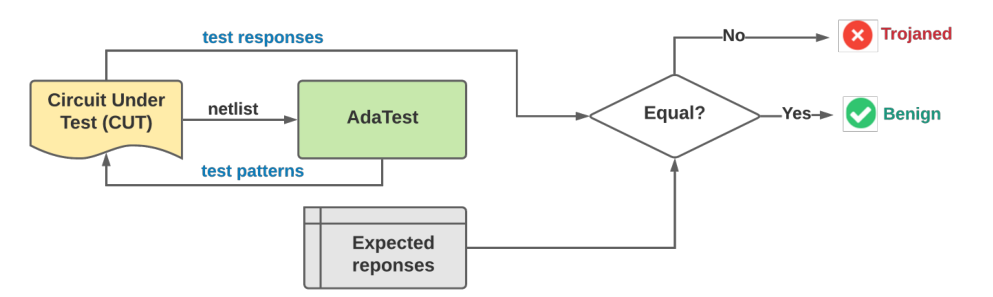
\includegraphics[width=0.75\textwidth]{./pictures/adatest.png}
  \caption{
    \textbf{Nota:} Circuit Under Test (Circuito bajo prueba), Expected responses
    (Respuestas esperadas), Test responeses (Prueba de respuestas) y Test
    patterns (Pruebas de patrón) son los elementos y sus salidas en inglés de
    la representación de Ada Test. Tomado de \cite{Chen2023}}
  \label{fig:adatest}
\end{figure} 

\begin{figure}[htb]
  \centering
  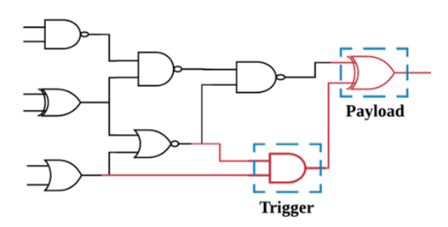
\includegraphics[width=0.75\textwidth]{./pictures/circuit.png}
  \caption{
    \textbf{Nota:} Este esquema es la demostración de un troyano de hardware.
    Tomado de \cite{Chen2023}}
  \label{fig:circuit}
\end{figure} 

\begin{figure}[htb]
  \centering
  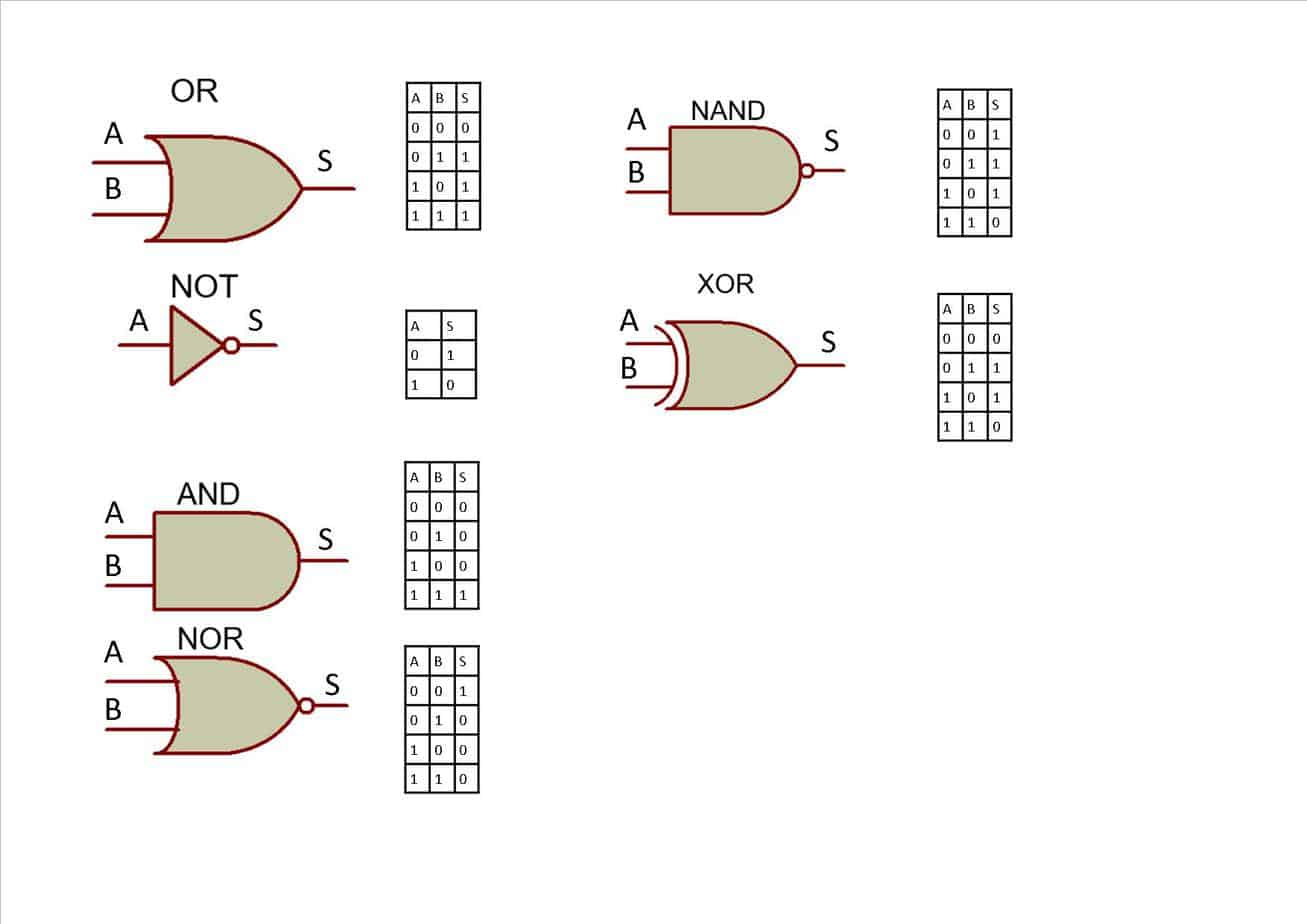
\includegraphics[width=0.75\textwidth]{./pictures/logic.png}
  \caption{
    Colección de las puertas lógicas y sus operaciones básicas dependiendo de la
    entrada que se le designe.
  }
  \label{fig:logic}
\end{figure} 

\subsection{Estado de los elementos de la ciberseguridad}

La manera en como se logra ver los conceptos de ciberseguridad, lo describe
\textcite{Mosquera2019} cuando trata de referirse a reducir los fallos que
puedan presenciarse gracias a las amenazas de la información de un activo (en
el contexto empresarial, se suele referir a los sistemas informáticos que
pertenecen a una organización y que pueden ser variados):
``La protección de activos de información, a través del tratamiento de amenazas
que ponen en riesgo la información que es procesada, almacenada y transportada
por los sistemas de información que se encuentran interconectados''
\parencite[Esic Business \& Marketing School, 2020, como se cita en][]{Bueno2022}

\subsubsection{
  Riesgos de seguridad e inteligencia artificial en los sistemas de salud
}

Por lo que se sabe, se piensa que cuando se tiene que implementar un sistema
inteligente, independientemente del tipo que sea, se sabe que puede ser
extremadamente útil para radiografías o identificación de patologías, pero se
sabe que esto puede conllevar a fallas desastrosas si se deja alguna brecha que
puede aprovechar un malware que rompa la cadena que lleva la red neuronal que
se emplea:

\begin{displayquote}
  Cabe recordar el artículo de 2010 de Dudzinski y sus colegas en el que se
  examinaban fallos puntuales -como lagunas en el control de infecciones, mal
  funcionamiento de la tecnología de desinfección, errores de laboratorio y
  clínicos incompetentes- que llegaron a afectar a miles de pacientes.
  \parencite{Banja2020}
\end{displayquote}

A esto se le suma al hecho de que también se puede añadir otros propósitos a la
información crítica de los usuarios, es decir, que se puede tomar esos datos
para utilizarlos para otros fines en lugar de los que son puestos.
\parencite{Banja2020}

\subsubsection{Manejo Legislativo}

Uno de los intentos que se realizaron a nivel nacional, fue el de mitigar los
ciberataques por medio de las normas del código penal colombiano, las cuales
condenan varias de las técnicas de ataque que afectan a los ciudadanos las
cuales incluyen suplantación de sitios web, robo de datos, hurto por medios
informáticos y otros delitos tratados por la ley. \parencite[Ley 1273 de 2009.
Por medio de la cual se modifica el Código Penal, se crea un nuevo bien jurídico
tutelado - denominado “de la protección de la información y de los datos”- y se
preservan integralmente los sistemas que utilicen las tecnologías de la
información y las comunicaciones, entre otras disposiciones. 5 de enero de 2009.
D.O. No. 47223, como se cita en][]{Mosquera2019}

Añadido a esto, nacionalmente se encontraron otras soluciones que se llevan
haciendo desde la popularización de la informática a nivel nacional, como por
ejemplo de que en las empresas se intente fomentar la seguridad de los equipos
pese a las circunstancias que se estén manejando para prevenir fallos en los
sistemas de información:

\begin{displayquote}
  Aparte de estos avances paulatinos, también debe tenerse en cuenta que en el
  transcurso de todo el año 2021, el Ministerio TIC, se empeñó en capacitar
  gratuitamente a PyMES (Pequeñas y Medianas Empresas) en materia de
  ciberseguridad, esto con el fin implementar acciones para proteger la
  información y para lograrlo era necesario que sus equipos de trabajo
  estuvieran en capacidad de enfrentar este reto y dar respuesta inmediata a
  cualquier tipo de amenaza.
  \parencite[MinTic, 2021, como se cita en][]{Bueno2022}
\end{displayquote}

\subsubsection{Tipos de malware}

En las revisiones de \textcite{Mosquera2019} se identificó la importancia de
hacer una revisión de los especímenes de malware a los que los servidores y
sistemas de cómputo individuales son atacados constantemente. Esto se hace,
puesto que esta situación por lo general, obliga a los desarrolladores a poner
mayor énfasis en la protección ante ciertos tipos de entradas maliciosas que
generan vulnerabilidades.

\begin{itemize}
  \item \textbf{Gusano:}
    Es semejante a un virus, la diferencia radica en que este se replica tanto
    en otro software como en la red sin necesidad de la supervisión de un
    usuario. \parencite{Rosli2019}

  \item \textbf{Troyano:}
    Es un malware que se presenta como un software legítimo; cumple la función
    de virus o gusano, solo que su principal fundamento es el uso del engaño de
    tal forma que un usuario piense que está usando un programa legítimo.
    \parencite{Rosli2019}

  \item \textbf{Botnet:}
    Es una red de computadoras infectadas, tales computadoras se les llaman
    ``bots'' los cuales cumplen las finalidades de un atacante, el cual logra
    acumular varios de estos ``bots'' a través troyanos o gusanos: ``Botnet
    también se define como una colección de ordenadores que han sido infectados
    por software malicioso y los convierte en bots, drones o zombis, que se han
    integrado en una colección mayor a través de una infraestructura
    centralizada de mando y control.'' \parencite{Rosli2019}

  \item \textbf{Ransomware:}
    Este tipo de malware busca encriptar toda la información en una máquina y
    luego hacer que el usuario inserte una clave para desencriptarla; las claves
    dadas por los atacantes requieren de una demanda otorgada por ellos, como
    pedir una cierta cantidad de dinero: ``Normalmente, una máquina infectada
    por ransomware queda ``congelada'', ya que el usuario no puede abrir ningún
    archivo, y la imagen del escritorio se utiliza para proporcionar información
    sobre las demandas de los atacantes.'' \parencite{Rosli2019}

  \item \textbf{Spyware:}
    Como su nombre lo dice, es un malware que se dedica a seguir al usuario de
    tal forma que este último no se dé cuenta del hecho. Se dedica
    principalmente a revisar los historiales de búsqueda, monitorear las
    actividades (para luego venderlas a terceros).
    \parencite{Rosli2019}
\end{itemize}

\subsubsection{Técnicas comunes de hacking}

% Insertar un parrafo introductorio a estas técnicas
% Meter otros conceptos

\begin{itemize}
  \item \textbf{Phishing:}
    Cuando una persona recibe un correo electrónico en el que un atacante se
    muestra como alguien importante, por norma general tienden a tentarse
    principalmente en hacer caso a las peticiones que se dan de tal forma que
    puedan aprovecharse del descuido generado por parte de los usuarios. Puede
    presentarse como un correo que hace una petición de credenciales, para que
    accedan a una página web de dudosa procedencia o para descargar malware
    asegurando que es solo un archivo de texto. De esa manera se logra ingresar al
    dispositivo de un usuario que la mitad del tiempo es incauto al llevarse por la
    impresión que genera el correo:

    \begin{displayquote}
      El delito con mayor crecimiento en el 2021, fue la violación de los datos
      personales, con un crecimiento de aproximadamente el 45\% con respecto al 2020,
      mediante la modalidad llamada ``phishing'' donde los cibercriminales realizan
      envíos masivos de emails adjuntando enlaces a páginas webs fraudulentas, así
      pueden llegar a infectar el dispositivo con un archivo adjunto malicioso o
      ``malware'' y de esta manera roban la información que necesitan.
      \parencite[INCIBE, 2010, como se cita en][]{Bueno2022}
    \end{displayquote}

    \iffalse
  \item \textbf{Ataques DDoS:}
    Chingar un equipo gigante que está para servir a montones de usuarios
    \fi

  \item \textbf{Vishing:}
    También conocido como el tráfico de datos personales, en este tipo de
    técnicas no se requiere de un malware, porque lo fundamental de esta
    técnica es el uso de la ingeniería social (engaño) para obtener información
    personal para ganar un beneficio monetario a través de sus datos.
    \parencite{Mosquera2019}

  \item \textbf{Uso de pirámides:}
    No se refiere literalmente a los polígonos tridimensionales, se refiere a
    una representación virtual de una estafa piramidal. Esto se logra sabiendo
    que en las criptomonedas hay incertidumbre en la legalidad y fluctuación,
    por lo que los inversionistas poco cuidadosos eventualmente compran una
    moneda virtual a unos estafadores que presumen ser expertos en tal economía.
    \parencite{Mosquera2019}

  \item \textbf{Suplantación de correo corporativo:}

  \item \textbf{Carding:}
    Como se intuye por el nombre, se refiere al robo de los datos de tarjetas de
    crédito o de débito, también con respecto a información financiera como las
    cuentas bancarias de una persona. Este tipo de técnicas se divide en varios
    métodos para obtener información, como el ``skimming'', el cual se resume en
    la clonación de tarjetas. \parencite{Mosquera2019}

  \item \textbf{Ofuscación:}
    Cuando se trata de leer un código de malware, para pasar desapercibido por
    un usuario, lo que se hace es ofuscarlo. Ofuscar un archivo significa
    modificarlo de tal forma que no pueda ser legible para cualquier usuario,
    esto a pesar de pasar desapercibido por cualquier usuario y antivirus, sigue
    siendo funcional cuando se ejecuta.
    \begin{displayquote}
      La imagen de memoria basada en opcodes puede tomarse para representar
      dinámicamente las actividades maliciosas. Aunque el malware ofuscado no
      puede ocultar cómo se comporta cuando se analiza dinámicamente, el
      análisis dinámico es incapaz de satisfacer todas las condiciones
      maliciosas para explorar todas las rutas de ejecución.
      \parencite{Aboaoja2022}
    \end{displayquote}
\end{itemize}

\subsubsection{Intentos de estudiar el malware}

Conociendo que cada vez se mejora la seguridad de los equipos de cómputo,
\textcite{Aboaoja2022} comenta que también se busca crear software malicioso que
realice sus funciones mientras no sea detectado. Por ende, para conocer las
funciones que realiza el programa, se realiza un proceso de análisis que se
caracteriza por tener tres tipos de acercamiento: Estático, dinámico e híbrido:
El primero consiste en estudiar el malware sin ejecutarlo, el segundo es
ejecutarlo para comprobar su comportamiento y el tercero, es usando las ventajas
que ofrecen los dos anteriores de acuerdo a los contextos (si el malware no
se puede analizar sin ejecutarlo, se puede usar el análisis dinámico, pero
siempre en un entorno que no esté conectado a internet y no cuente con
información crítica del usuario)

Estos tipos de análisis logran obtener ciertos tipos de datos, en los cuales se
puede tomar en consideración la metodología de análisis más correcta de acuerdo
a una situación en particular; por ejemplo, si se tiene un malware que realiza
una serie de llamadas API, resulta más conveniente usar el análisis dinámico,
ya que por medio de este se logra comprender directamente cuáles son las
herramientas del sistema que tiene por defecto. Del mismo se aplica para
archivos que están pensados para escalar privilegios dentro del sistema, como lo
pueden ser las bibliotecas de enlace dinámico (archivos con código ejecutable
que se cargan según la necesidad de un programa) o archivos portables (la
estructura más común para archivos ejecutables)
\parencite{Aboaoja2022}

Aparte de estos modelos de análisis de malware, lo que se necesita evidentemente
antes de provocar errores inesperados por parte de la operación de algún
malware, lo que se hace dependiendo del tipo de malware es usar unos modelos de
detección. Estos modelos son basados en firma, comportamiento, heurístico y
discusión. \parencite{Aboaoja2022}

A continuación, se hace una descripción de tales modelos según la información
otorgada por los mismos autores:

\begin{itemize}
  \item \textbf{Modelo basado en firma}
    El modelo basado en firma, consiste en encontrar un patrón muy común en
    archivo con código ejecutable, es muy frecuente que sea automatizado por
    los programas antivirus, ya que estos comparan las firmas que tienen según
    la base de datos en donde se encuentra vinculados para evitar más
    comportamientos semejantes.

  \item \textbf{Modelo basado en comportamiento}
    Como bien se intuye, lo que se hace es ejecutar el código del malware en un
    entorno asegurado, concretamente en una máquina virtual. Las máquinas
    virtuales son simuladores de sistemas operativos completamente funcionales,
    pero cuya información no está relacionada con la del disco duro del usuario.

  \item \textbf{Modelo basado en heurística}
    Una vez extraída la información, lo que se hace primero es generar una
    serie de reglas genéricas que pueden ser también generadas por una
    inteligencia artificial (La herramienta YARA realiza tales acciones
    basándose en los aprendizajes no supervisados de Machine Learning). Luego
    con esas reglas, se investiga el contenido del malware empleando las
    técnicas estáticas y dinámicas.

  \item \textbf{Modelo basado en discusión}
    Como las desventajas de los análisis del malware se hacen presentes al
    aplicarlos en archivos con código ofuscado y con comportamientos poco
    predecibles, se considera entonces que es una situación en discusión. En
    otras palabras, las técnicas a emplear no son suficientes para conocer las
    características del malware y se tienen que descubrir para realizar otras
    acciones.
\end{itemize}

\subsubsection{Líneas de tiempo acorde a los tópicos}

\begin{figure}[hb!]
  \centering
  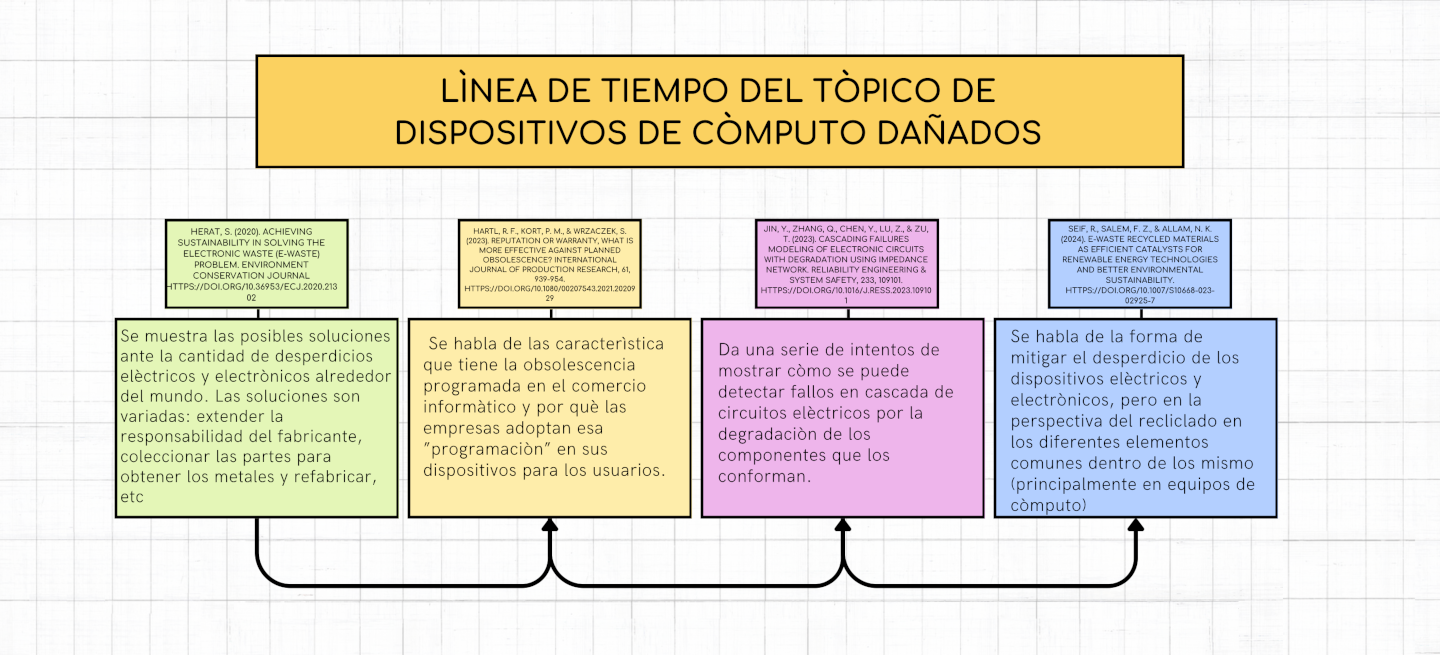
\includegraphics[width=1\textwidth]{./pictures/timeline_1.png}
  \caption{Línea de tiempo del tópico de dispositivos de cómputo dañados}
  \label{fig:timeline1}
\end{figure} 

\begin{figure}[ht!]
  \centering
  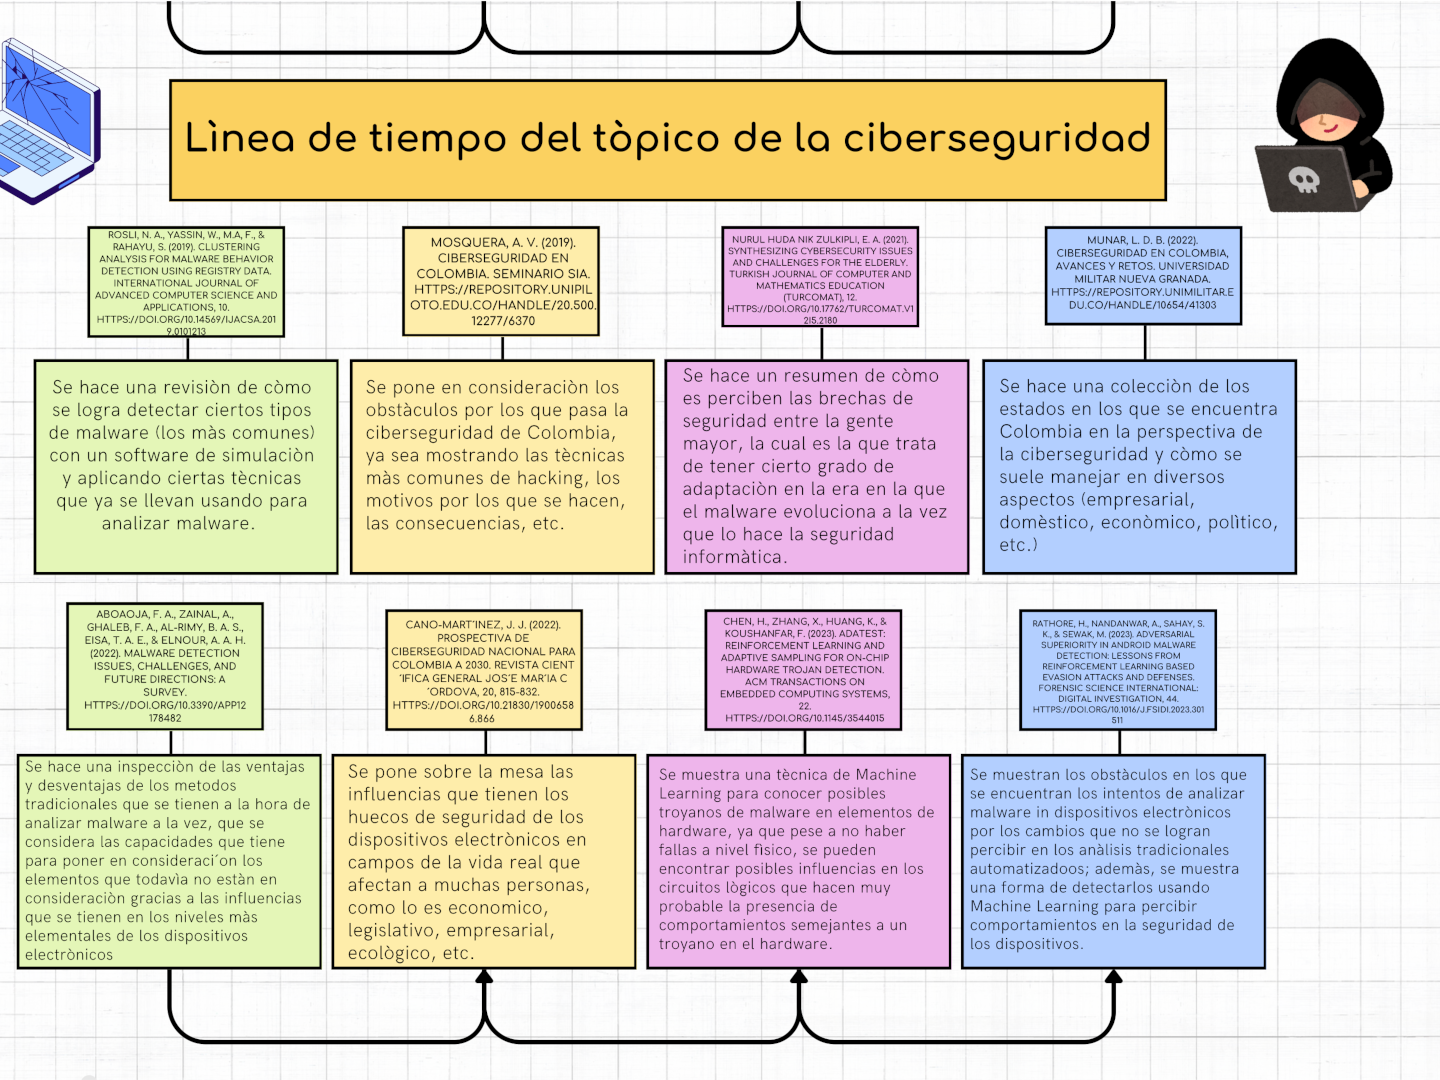
\includegraphics[height=0.5\textheight]{./pictures/timeline_2.png}
  \caption{Línea de tiempo del tópico de la ciberseguridad}
  \label{fig:timeline2}
\end{figure} 

\begin{figure}[hb!]
  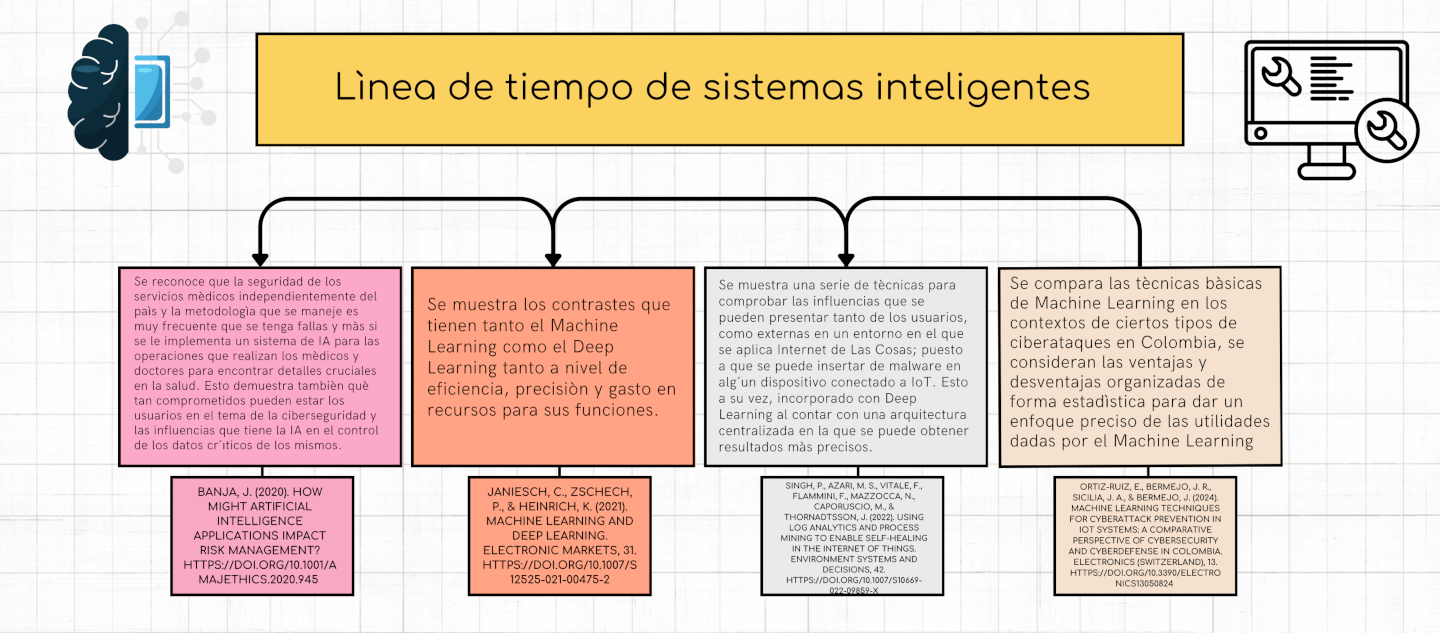
\includegraphics[width=0.85\textwidth]{./pictures/timeline_3.png}
  \caption{Línea de tiempo de sistemas inteligentes}
  \label{fig:timeline3}
\end{figure} 

\begin{figure}[ht!]
  \centering
  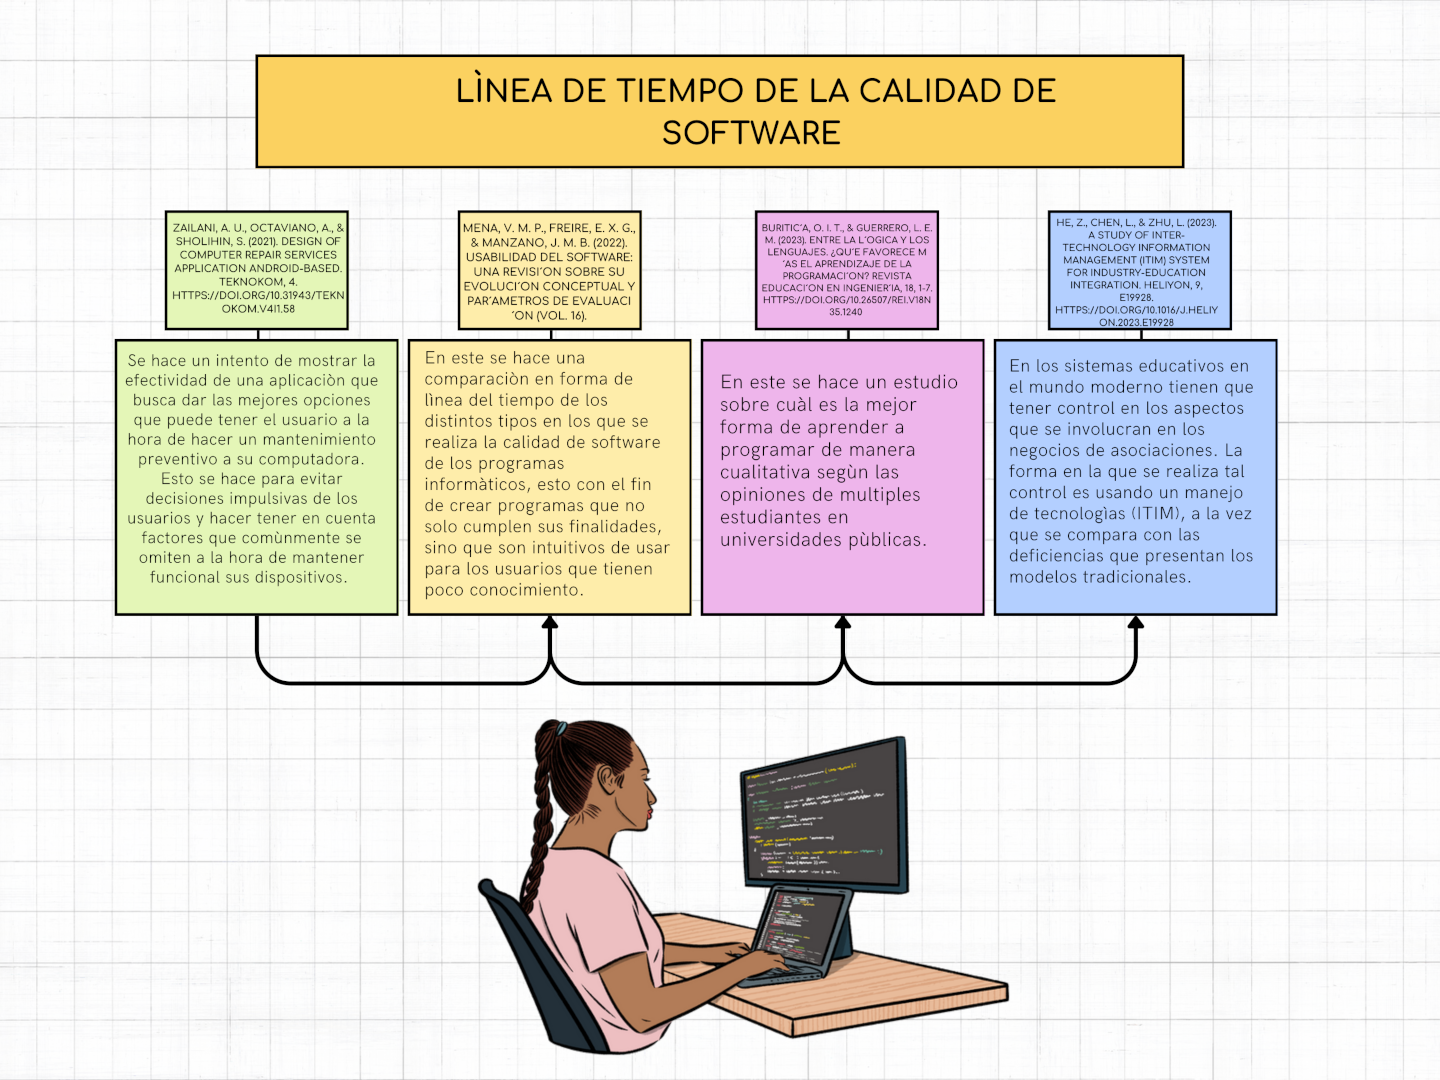
\includegraphics[width=1\textwidth]{./pictures/timeline_4.png}
  \caption{Línea de tiempo de la calidad de software}
  \label{fig:timeline4}
\end{figure} 

\pagebreak
\section{Pregunta generadora}

En la búsqueda de información sobre nuestra problemática, se propuso la creación
de un software que se dedique a otorgarle a un usuario la mejor acción que puede
realizar para prevenir fallos de su computadora para que pueda realizar las
acciones que necesita en su día a día. Pero en esas circunstancias, se planteó
una pregunta que resulta ser el común denominador de los campos que involucra el
software: ¿Qué elementos hay que tener en cuenta para desarrollar el software?

Esta pregunta lo que lleva a un desarrollador es a indagar sobre los conceptos
en lo que es sumamente fatuo para posteriormente, tener un esquema lo
suficientemente satisfactorio en el sentido de que se pueda dar a conocer las
respuestas ante las incógnitas que se genera: Como el qué hacer para crear un
sistema inteligente sea capaz de distinguir entre acciones bajo la condición del
usuario y las de agentes externos, o cómo comparar rendimientos en diferentes
periodos de acuerdo al uso y qué consejos puede dar al usuario de tal modo que
no se encuentre con problemas e incógnitas a la hora de solucionar tal
situación.

Y una de las preguntas que formuló \textcite{Trejos2023} para conocer cuál es la
mejor manera de aprender a programar en entornos académicos, como lo son el de
una universidad pública: ``¿Qué favorece más en el aprendizaje de la
programación: los fundamentos matemáticos y lógicos o los lenguajes de
programación?'' De esta pregunta nos lleva a pensar en el contexto de realizar
un mantenimiento preventivo en el hardware y software como el preguntarnos sobre
cuáles son los medios indicados para dar los resultados que se espera hacia los
usuarios. Y sobre todo, para hacerlos lo suficientemente rápidos como para
satisfacer las necesidades actuales.

\pagebreak
\section{Objetivos}
\subsection{Objetivo general}

Crear una aplicación que tendrá dos finalidades, donde se combinará el
mantenimiento preventivo de hardware y la ciberseguridad para garantizar un
funcionamiento óptimo y seguro de los equipos de cómputo.

\subsection{Objetivos específicos}

\begin{itemize}
  \item
    Desarrollar un sistema de diagnóstico (basado en Ada Test) que permita
    identificar los problemas leves de hardware antes de se generen daños
    críticos.

  \item
    Implementar en las técnicas de ciberseguridad los elementos de inteligencia
    artificial para la detección de ligeras perturbaciones en archivos.

  \item
    Diseñar una interfaz lo suficientemente fácil de usar para el mantenimiento
    preventivo del equipo.

  \item
    Crear un sitio web para la publicación del software con interfaz gráfica
    con guía adjuntada.
\end{itemize}

\pagebreak
\section{Solución}

Normalmente, cuando se piensa en el tema del malware, de la seguridad, de la
optimización del rendimiento de un computador y asegurar una garantí mayor,
directamente se asume como solución el uso de un antivirus. En el caso de las
PyMES se le incorporaría la acción de concientización a partir de conferencias
para hacer una gestión de todo lo que se está haciendo y como se refiere
\textcite{Bueno2022}, aplicar una décima parte del presupuesto. Y en el caso de
los usuarios domésticos, estos deben tener cierta cultura de los elementos que
tiene su máquina, para saber las acciones inmediatas ante un problema menor y
aplicarlas de forma sabia sin necesidad de gastar dinero en reparaciones junto
con licencias a las que se les debe pagar en un cirtos periodos de tiempo para
su uso.

Por lo tanto, se pensó en la idea de crear un software inspirado en los
programas antivirus y con Ada Test incorporado para prevenir fallos
catastróficos sin el conocimiento de los usuarios. Estas herramientas con las
características dadas por \textcite{Chen2023}, \textcite{Ortiz2024} y
\textcite{Zailani2021}, se pueden utilizar para crear un software ayudar a
identificar elementos que hacen ligeras perturbaciones en los archivos y que
conllevan a que se puedan generar vulnerabilidades que generen los efectos
explicados por \textcite{Mosquera2019} y \textcite{Rosli2019}. Este software a
su vez se deja disposición una versión gratuita y una de pago, sin necesidad de
recurrir a la atención en anuncios en plena ejecución de la aplicación, que
como comenta \textcite{Hartl2023} es molesto. 

La versión de pago estará dedicada a funcionalidades más sofisticadas que las
que ofrece el software gratuito, es decir aquellas que \textcite{Singh2022} y
\textcite{Waqar2023} comentan para dispositivos de internet de las cosas.
Esto es así, puesto que aunque el IoT cada vez se hace más presente, en el uso
doméstico es poco común, bastante costoso y que puede tener mayor influencia
de problemas de brechas de seguridad expuestas por \textcite{Rosli2019}. Y como
el Deep Learning requiere de una maquinaria pesada, es necesario contar con
base monetaria para mantenerla y seguir puliendo la detección de malware.

Esta noción fue inspirada por los elementos presentados por
\textcite{Aboaoja2022} al intentar realizar un análisis con el malware que
evoluciona con el paso del tiempo y que influye en aspectos que indirectamente
están relacionados con la informática, y ni hablar lo que ocurre a nivel
nacional según \textcite{CanoMartinez2022}.

Para crear el software de una forma para los usuarios que cuentan con un
inadecuado funcionamiento de un equipo de cómputo, se tiene que disponer de un
medio intuitivo que cumpla con las características otorgadas por
\textcite{Mena2022} de tal forma que cumpla no solo con la calidad del software
ante los usuarios, sino también para que sea útil para aquellos que usan el
software a desarrollar del mantenimiento preventivo:

\begin{displayquote}
  La usabilidad pasó a ser un factor para medir la calidad de un producto de
  software, pues se debe garantizar la eficiencia, eficacia, satisfacción en el
  uso del producto y su relación con los usuarios; por lo que llega a ser
  considerada fuertemente en el área del diseño de interfaces y la interacción
  humano computador, para buscar la facilidad de uso de un producto.
\end{displayquote}

Y en lo que se revisó de \textcite{Trejos2023}, se concluyó que el uso del
lenguaje de programacón Java sería útil para la creación de una interfaz que
caracteriza su usabilidad, y el uso del lenguaje de programación C para tener
control tanto de los elementos de bajo en la perspectiva de alto nivel. Y 
sabiendo que tales lenguajes representan una oportunidad para usar Ada Test para
beneficiar a los usuarios que cuenten con un equipo que funciona de forma
deficiente.

\pagebreak
\section{Conclusiones}

Tras haber hecho una revisión de lo que se encontró con respecto a cómo se
maneja tanto la ciberseguridad como el mantenimiento preventivo de los
computadores, se aprendió que para dar un aporte contundente a los usuarios que
buscan proteger su máquina sin gastar tanto dinero, se necesita entonces una
colección amplia de elementos y técnicas para realizar tal acción. A su vez,
se tiene en cuenta de que las tecnologías cada vez avanzan más rápido de lo que
nosotros podemos aprender de forma individual, ya que por la globalización
alguien del que no conocemos pueda estar a pasos adelantados en cuanto a
conocimiento.

Para los usuarios que tienen un equipo que funciona de forma deficiente, es
bastante extraño conocer sus orígenes, por lo que se piensa que tiene que
encontrar una forma más amigable de hacer visibles todos estos problemas;
incluyendo los componentes internos de los computadores actuales, al ser estos
complejos. Las deficiencias como la conexión a internet muy lenta, el
almacenamiento tanto temporal como permanente que resultan ser problemáticos,
los anuncios molestos sin el navegador abierto y demás, hacen de la
experiencia de uso para los usuarios desesperante (incluso para los que tienen
poca voluntad de tener control sobre estos).

Los problemas tanto del desgaste de los componentes electrónicos, la instalación
poco apropiada de los elementos físicos del computador, la falta de rigurosidad
en la seguridad en la perspectiva de los programas y de la susceptibilidad al
engaño, hacen que directamente los sistemas de cómputo reflejan directamente tal
problemática. Para atender a este tipo de problemas, resulta abrumador por los
elementos que se acaban de aprender y sobre todo, porque va más allá del control
que tenemos comúnmente con los computadores, es decir que implica a que nosotros
tengamos una noción amplia en elementos de bajo nivel y de la electrónica con la
que se sustenta la información actual.

En esta era, la maquinaria cibercriminal puede volverse más avanzada de lo que
se utiliza actualmente en la ciberseguridad, y como el tema de la inteligencia
artificial se está haciendo cada vez más y más conocido entre la gente, se puede
conocer otras técnicas y otros conceptos que se pueden originar debido a las
ventajas que representan a la hora de buscar información. Todo, con tal de 
seguir haciendo que un computador continúe funcionando acorde a nuestras
necesidades.

\printbibliography
\end{document}
